\subsection{Recurrent Neural Networks}
Recently, the application of deep learning in cosmological research is very extensive and successful. Following the work of \cite{escamilla2020deep}, we reconstruct the distance moduli from the Pantheon compilation \cite{scolnic2018complete} with RNN+BNN. In this process, the reconstruction of distance only depends on the dataset, and without any assumption on the cosmological model.

RNN is a class of nets which can predict the future from the complex sequential information without any model assumption, but is incapable of estimating the uncertainty of target. This shortcoming can be fixed up with BNN. Therefore, our neural network is composed of RNN and BNN, the details of which are described bellow.

Handling long sequences, the training of RNN will take a long time and the information of initial inputs will gradually fades away. Thus, we adopt the time step $t=4$ to alleviate the long training time, and use the most popular basic cell called Long Short-Term Memory (LSTM) cell to solve the problem of information loss. RNN with LSTM cell is aware of what to store, throw away and read. The architecture of LSTM is shown in Figure \eqref{lstm_cell}. In the unrolled RNN, the neurons at each time step $t$ receive the inputs as well as the outputs from the previous time step. In the neural network, the loss function is used to depict the difference between the targets and the predicts. We adopt the Mean Squared Error (MSE) function as the loss function and find the minimum with the Adam optimizer.

\subsubsection{LSTM Cell}
\begin{figure} [H]
	\centering
	\includegraphics[width=\textwidth]{lstm_Cell}
	\caption{Neural Network Architecture}
	\label{lstm_cell}
\end{figure}

The computations of LSTM are
\begin{align}
i^{<t>}=\sigma\left(W_{x i}^{T} \cdot x^{<t>}+W_{h i}^{T} \cdot h^{<t-1>}+b_{i}\right) \\
f^{<t>}=\sigma\left(W_{x f}^{T} \cdot x^{<t>}+W_{h f}^{T} \cdot h^{<t-1>}+b_{f}\right) \\
o^{<t>}=\sigma\left(W_{x o}^{T} \cdot x^{<t>}+W_{h o}^{T} \cdot h^{<t-1>}+b_{o}\right) \\
g^{<t>}=A_{f}\left(W_{x g}^{T} \cdot x^{<t>}+W_{h g}^{T} \cdot h^{<t-1>}+b_{g}\right) \\
c^{<t>}=f<t>\otimes c^{<t-1>}+i^{<t>} \otimes g^{<t>}, \\
y^{<t>}=h^{<t>}=o^{<t>} \otimes A_{f}\left(c^{<t>}\right),
\end{align}
where $\sigma$ is the sigmoid function that outputs a value between 0 and $1, t$ is the time step referring to the current sequence (for example $t=1$ for the first redshift). The superscript $<t>$ indicates a vector of steps $t$, the superscript $T$ is the transpose of the matrix, the dot is matrix product and $\otimes$ is direct product. $x^{<t>}$ and $y^{<t>}$ are respectively the current input and output vectors. $h<t>$ and $c^{<t>}$ are respectively the short-term state and long-term state of LSTM cells. $A_{f}$ is an activation function to make the network be capable of solving complex tasks by introducing the non-linearity to network. In our work, we use the tanh activation function, which is defined as
$$
A_{f_{\operatorname{Tanh}}}=\tanh (x)=\frac{e^{x}-e^{-x}}{e^{x}+e^{-x}} .
$$

\subsubsection{Network Architecture}
\begin{figure} [H]
	\centering
	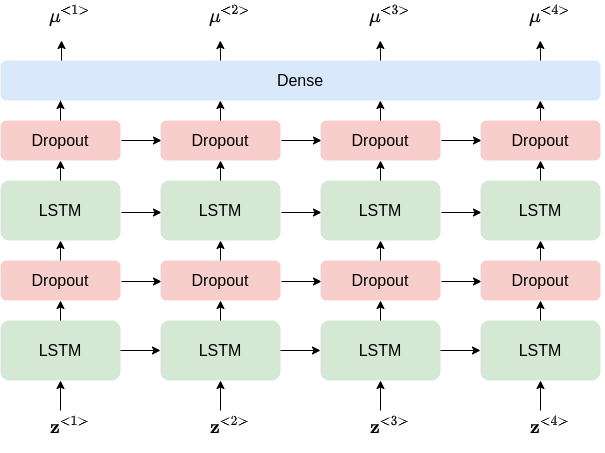
\includegraphics[width=\textwidth]{network_arch}
	\caption{Neural Network Architecture}
	\label{newtork_arch}
\end{figure}

The architecture of our network \eqref{newtork_arch}, with one hidden layer (left), unrolled through time step $t=4$ (right). In the unrolled network, each column is one of the $t$ time steps, while the three rows from bottom to top represent input layer, hidden layer and output layer, respectively. The first two layers with tanh activation function consist of LSTM cell containing 100 neurons, while the output layer is a fully-connected (dense) layer. To avoid overfitting, the dropout technique is employed between LSTM and its next layers, and we set the dropout rate to $0.2$.


There are four connected layers playing different roles, where the main layer that outputs $g^{<t>}$ analyzes the current inputs $x^{<t>}$ and the previous state $h^{<t-1>}$, the rest three layers are gate controllers: (a) Input gate controlled by $i^{<t>}$ determines which parts of $g^{<t>}$ should be added to $c^{<t>}$, (b) Forget gate controlled by $f<t>$ determines which parts of $c^{<t>}$ should be abandoned, (c) Output gate controlled by $o<t>$ determines which parts of $c<t>$ should be output. It can be easily found that, these gate controllers are related to the logistic activation function $\sigma$, thus they would close the gate if output 0 and open it if output $1 . W_{x i}, W_{x f}, W_{x o}$ and $W_{x g}$ are the weight matrices of each of above four layers connecting to the input vector. $W_{h i}, W_{h f}, W_{h o}$, and $W_{h g}$ are the weight matrices of each of layers connecting to the previous short-term state. $b_{i}, b_{f}, b_{o}$, and $b_{g}$ are the bias terms for each of layer.

In a deep neural network, the training may suffer from overfitting due to a large number of its own hyperparameters. We can use the method called regularization to prevent it from overfitting. Dropout is one of the most popular regularization techniques, applying in some layers to reduce the overfitting risk. In this way, some neurons has a probability of being ignored at every step controlled by dropout rate. Besides, it is also of benefit to estimate the confidence of the training in BNN.

\subsubsection{Bayesian Neural Networks}
BNN is a supplementary of RNN for calculating the uncertainty of the prediction. BNN is defined in terms of a prior distribution with parameters over the wights $p(\omega)$, which manifests a prior belief about parameters generating the observations. With a given dataset $\{\mathbf{X}, \mathbf{Y}\}$, we can achieve the posterior distribution of the parameters space $p(\omega \mid \mathbf{X}, \mathbf{Y})$. Thus the output of a new input point $x$ can be anticipated by the integration
$$
p\left(y^{*} \mid x^{*}, \mathbf{X}, \mathbf{Y}\right)=\int p\left(y^{*} \mid x^{*}, \omega\right) p(\omega \mid \mathbf{X}, \mathbf{Y}) \mathrm{d} \omega
$$
A full BNN is extremely complex. However, \cite{gal2016theoretically} developed a new framework casting dropout training in deep neural network as approximate Bayesian inference in deep Gaussian processes and successfully applied in RNN. Their results offer a Bayesian interpretation of the dropout technique, and verify that a network with a dropout is mathematically equivalent to the Bayesian model. When the RNN is well-trained and executed $n$ times, the network is equivalent to BNN. Therefore, we employ the dropout in the training and call the trained network $n$ times to estimate the uncertainty of outputs, where the dropout is an approximation of the Gaussian processes and cooperates with the activation function to determine the confidence regions of prediction.